\section{Spannung, Strom und Widerstand}
\subsection{Kraft zwischen Punktladungen}
Massen zeihen sich durch Gravitation an. Der Betrag der Anziehungskraft zwischen zwei punktförmigen Massen $m_1$ und $m_2$ im Abstand $d$ ist
\begin{equation}
\boxed{F_G=G\cdot \dfrac{m_1\cdot m_2}{d^3}}
\end{equation}
Geladene Körper üben zusätzliche Kräfte aus. Diese Kräfte werden Coulombsche Kräfte genannt, wobei sich Ladungen mit gleichem Vorzeichen abstossen und mit unterschiedlichen Vorzeichen anziehen.
\newline\newline
Das Coulombsche Kraftgesetz für zwei Punktladungen $Q_1$ und $Q_2$ mit Permittivität des Mediums $\epsilon$ lautet
\begin{equation}
\boxed{F_C=\dfrac{1}{4\pi \epsilon}\cdot \dfrac{Q_1\cdot Q_2}{d^2}}
\end{equation}
\subsection{Das Feld}
Der Betrag der Kraft nimmt quadratisch mit dem Abstand ab. Jede Ladung verändert in ihrer Umgebung den Zustand des Raumes derart, dass auf andere Ladungen Kraftwirkungen ausgeübt werden. Dieser Zustand des Raumes bezeichnet man als \textbf{elektrisches Feld}. Das elektrische Feld wird in jedem Raumpunkt durch einen Vektor $\overrightarrow{E}$ beschrieben, der in Richtung der Kraftweist, die das elektrische Feld auf eine positive Probeladung $q_2$ ausübt.
\begin{equation}
\boxed{\overrightarrow{E}=\dfrac{\overrightarrow{F}}{q_2}}
\end{equation}
Setzt man das \textbf{Coulombsche Kraftgesetz} für die Feldstärke ein, so erhält man für die elektrische Feldstärke derPunktladung $Q_1$, wobei $\overrightarrow{e}_r$ der Einheitsvektor in Richtung $\overrightarrow{r}$ und $r$ der Abstand vom $Q_1$. Im Feldmodell ist eine Punktladung $Q$ von einem elektrischen Feld $E$ umgeben, das den ganzen Raum durchdringt.
\begin{equation}
\boxed{\overrightarrow{E}\left(\overrightarrow{r}\right)=\overrightarrow{e}_r\cdot \dfrac{Q_1}{4\pi\epsilon r^2}}
\end{equation}
\newline\newline
Stellt man Kräfte auf Ladungen fest, so ist die Ursache ein \textbf{elektrisches Feld}. Stellt man Kräfte auf Massen fest, so ist die Ursache ein \textbf{Gravitationsfeld}.
\newline\newline
Durch Feldlinien werden elektrische Felder dargestellt. Diese geben in jedem Raumpunkt die Richtung des Feldvektors an. Solche Feldbilder vermitteln einen anschaulichen Überblick über den Verlauf des Feldes.
\subsection{Arbeit im Feld, Spannung und Potential}
Für die Verschiebung von Massen im Gravitationsfeld (i.d.R. Potentialfeld) benötigt man Arbeit. Die zu leistende Arbeit von einem Punkt $A$ nach $B$ ist nicht vom Weg abhängig, sondern nur von der Höhendifferenz zwischen $A$ und $B$.
\begin{equation}
\boxed{W_{AB}=\displaystyle \int_{P_A}^{P_B}\overrightarrow{F}\bullet \text{d}\overrightarrow{s}=q\cdot \underbrace{\displaystyle\int_{P_A}^{P_B}\overrightarrow{E}\bullet \text{d}\overrightarrow{s}}_{U_{AB}}}
\end{equation}
Diese wegunabhängige Arbeit führt zu der Definition der \textbf{elektrischen Spannung}, nämlich Arbeit pro Ladung.
\begin{equation}
\boxed{U_{AB}=\dfrac{W_{AB}}{q}}
\end{equation}
Für die Spannung $U_{AB}$ wird ein gerichteter Spannungspfeil eingetragen. Der Pfeil erinnert an das Wegintegral für die Arbeit. So ist die Spannung $U_{AB}$ der von $A$ nach $B$ zeigt.
\newline\newline
Mit der Spannung wird das elektrische Potential eingeführt. Die Spannung wird durch zwei Punkte angegeben, das Potential hingegen wird einem Punkt im Raum zugeordnet. Für die Einführung des Potentials wird ein Punkt im Raum zum sogenannten \textbf{Potentialnullpunkt} bzw. \textbf{Bezugspunkt} erklärt und von diesem Punkt wird die Spannung gemessen. Die Wahl des Bezugspunktes mit $V=0$ ist willkürlich. Für den Zusammenhang zwischen Spannung und Potential gilt folgende \textbf{Potentialdifferenz}, wobei Potential und Spannung dieselbe Einheit Volt $\left([U]=[V]=V\right)$ haben.
\begin{equation}
\boxed{
\begin{array}{lll}
U_{AB}=V_A-V_B&=&-\displaystyle \int_{P_0}^{P_A}\overrightarrow{E}\bullet \text{d}\overrightarrow{s}+\displaystyle \int_{P_0}^{P_B}\overrightarrow{E}\bullet \text{d}\overrightarrow{s}\\
&=&\displaystyle \int_{P_A}^{P_0}\overrightarrow{E}\bullet \text{d}\overrightarrow{s}+\displaystyle \int_{P_0}^{P_B}\overrightarrow{E}\bullet \text{d}\overrightarrow{s}=\displaystyle \int_{P_A}^{P_B}\overrightarrow{E}\bullet \text{d}\overrightarrow{s}
\end{array}
}
\end{equation}
Liegt eine Ladung $q$ im Punkt $P$, der das Potential $V\left(P\right)$ aufweist, so ergibt folgendes Produkt die potentielle Energie der Ladung gegenüber dem Potentialnullpunkt
\begin{equation}
\boxed{E_{\text{pot}}=q\cdot V\left(P\right)}
\end{equation}
\subsection{Strom}
Die Bewegung von elektrischen Ladungsträgern ist der \textbf{elektrische Strom} bzw. \textbf{Ladungsfluss} von Ladungsträger. Die Richtung eines positiven Stromes ist so definiert, dass er von der Elektrode höheren Potentials zur Elektrode niedrigeren Potenttials fliesst. Innerhalb der leitenden Verbindung hat er die gleiche Richtung wie die elektrische Feldstärke. In einem Leiter, durch dessen Querschnitt die Ladung $Q=n\cdot e$ in der Zeit $t$ hindurchtritt, ist die Stromstärke $I$ definiert als
\begin{equation}
\boxed{I=\dfrac{Q}{t}}
\end{equation}
Einen solchen zeitlich konstanten Strom nennt man \textbf{Gleichstrom}. Einheit der elektrischen Stromstärke ist das Ampere $([I]=\text{A})$. Bezogen auf die Fläche $A$, durch die Strom tritt, ist ferner die \textbf{Stromdichte}
\begin{equation}
\boxed{J=\dfrac{I}{A}}
\end{equation}
Die nicht zeitlich konstanter elektrische Stromstärke ist definiert als die \textbf{momentane Stromstärke} bei einem beliebigen Zeitpunkt $t$
\begin{equation}
\boxed{i\left(t\right)=\displaystyle \lim_{\triangle t\rightarrow 0}\dfrac{\triangle Q}{\triangle t}=\dfrac{\text{d}q\left(t\right)}{\text{d}t}}
\end{equation}
Man ordnet dem elektrischen Strom eine positive Zählrichtung zu, welche der Bewegungsrichtung positiver Ladungsträger im Leiter entsprechen würde, also vom Pluspol zum Minuspol, und kennzeichnet diese positive Zählrichtung durch einen entsprechenden Zählpfeil.
\newline\newline
Die positive Zählpfeilrichtung des Stromes ist ausserhalb einer Energiequelle vom Pluspol zum Minuspol festgelegt und entspricht der Bewegungsrichtung positiver Ladungsträger.
\subsection{Widerstand}
Jeder Leiter setzt dem Stromfluss einen elektrischen Widerstand entgegen. Hat ein Verbraucher zwei Anschlussklemmen so bildet er einen \textbf{Zweipol}. Schliesst man eine Spannung $U$ an die Zweiklemmen so wird ein Strom $I$ durch den Zweipol fliessen. Je grösser der Strom desto grösser die Spannung. Den Widerstand eines Zweipols bezeichnet man als linear und heisst \textbf{ohmsches Gesetz}
\begin{equation}
\boxed{R=\dfrac{U}{I}=\dfrac{1}{G}}
\end{equation}
So ist $R$ der elektrische Widerstand und $G$ der elektrische Leitwert des Zweipols, wobei beide konstant sind. Sind $R$ und $G$ nicht konstant, so sind beide strom- und spannungsabhängig. Die Strom-Spannungskennlinie verläuft nichtlinear. Der Quotient $u/i=f\left(i\right)$ ergibt einen nichtlinearen Widerstand und man erhält einen \textbf{differentiellen Widerstand}.
\begin{equation}
\boxed{r=\dfrac{\triangle u}{\triangle i}\Longrightarrow \dfrac{\text{d}u}{\text{d}i}}
\end{equation}
Die Einheit des Widerstandes ist das Ohm $\left(\Omega\right)$ und die Einheit des elektrischen Leitwerts ist das Siemens $\left(\text{S}\right)$ oder $\left(\Omega^{-1}\right)$.
\subsection{Spezifische Leitfähigkeit und spezifischer Widerstand}
Der elektrische Widerstand ist eine \textbf{Materialgrösse}, d.h. $R\approx l/A$. Für einen linearen Leiter der Länge $l$ mit dem überall gleichen Querschnitt $A$ erhält man
\begin{equation}
\boxed{R=\dfrac{\rho\cdot l}{A}=\dfrac{l}{\sigma\cdot A}}
\end{equation}
So ist $\rho$ mit Einheit $\left([\rho]=\Omega\,\text{m}\right)$ der spazifische Widerstand und $\sigma$ mit Einheit $\left([\sigma]=\text{S}\,\text{m}^{-1}=\Omega^{-1}\,\text{m}^{-1}\right)$ der spezifische Leitwert oder die Leitfähigkeit des Leitermaterials.
\newline\newline
Häufigste Leitwerkstoffe sind Kupfer und Aluminium. Für Kontakte werden Gold, Silber und Wolfram eingesetzt und für Heizleiter Chromnickel. Für Messwiderstände werden Manganin und Konstatan wegen ihrer thermischen Eigenschaften verwendet. Der elektrische Widerstand eines Leiters ist temperaturabhängig $R=f\left(\theta\right)$.
\newline\newline
Die nichtlineare Temperaturen wird für den unteren Bereich bis $200^{\circ}\,\text{C}$ mit folgendem Ansatz linearisiert, wobei $R_{20}$ der Widerstandswert bei $20^{\circ}\,\text{C}$, $R_W$ der Widerstandswert bei der Temperatur $\theta_W$, $\theta_W$ die Temperatur des Widerstandes in $^{\circ}\,\text{C}$ und $\alpha_{20}$ der Temperaturkoeffizient in $1/^{\circ}\,\text{C}$
\begin{equation}
\boxed{R_{\text{W}}=R_{20}\cdot \Big[1+\alpha_{20}\cdot \left(\theta_W-20^{\circ}\,\text{C}\right)\Big]}
\end{equation}
Für höhere Temperaturen ab $200^{\circ}\,\text{C}$ wird zusätzlich noch ein quadratischer Term in der Näherung eingefügt, wobei $\beta_{20}$ der Temperaturkoeffizient in $\left(1/^{\circ}\,\text{C}\right)^2$
\begin{equation}
\boxed{R_{\text{W}}=R_{20}\cdot \Big[1+\alpha_{20}\cdot \left(\theta_W-20^{\circ}\,\text{C}\right)+\beta_{20}\cdot \left(\theta_W-20^{\circ}\,\text{C}\right)^2\Big]}
\end{equation}
Somit sind $\alpha_{20}$ und $\beta_{20}$ temperaturabhängig. Die meisten häufig eingesetzten Metalle haben einen Temperaturbeiwert in der Nähe von $\alpha=0.004\,\text{K}^{-1}$. Widerstände ändern bei einer Temperaturänderung um je $1\,\text{K}$ ihren Wert um etwa $0.4\,\%$.
\begin{table}[H]
\centering
\begin{tabular}{ccc}\hline
\textbf{Material}&\textbf{Typ}&\textbf{$\sigma$ / $\Omega^{-1}\text{m}^{-1}$}\\\hline
Quarz &Isolator&$\approx 10^{-17}$\\
Silikonöl&Isolator&$\approx 10^{-15}$\\
Mica&Isolator&$\approx 10^{-15}$\\
Paraffin&Isolator&$\approx 10^{-15}$\\
Hartgummi &Isolator&$\approx 10^{-15}$\\
Porzellan&Isolator&$\approx 10^{-14}$\\
Glas&Isolator&$\approx 10^{-12}$\\
Bakelit&Isolator&$\approx 10^{-9}$\\
Destilliertes Wasser&Isolator&$\approx 10^{-4}$\\
Sandige Erde, trocken &schlechter Isolator&$\approx 10^{-3}$\\
Feuchte Erde &schlechter Isolator&$\approx 10^{-2}$\\
Frischwasser &schlechter Isolator&$\approx 10^{-2}$\\
Tierisches Fett&schlechter Isolator&$\approx 4\cdot 10^{-2}$\\
Tierischer Muskel &schlechter Leiter&$0.4$\\
Tierisches Blut &schlechter Leiter&$0.7$\\
Germanium (rein)&Halbleiter&$\approx 2$\\
Meerwasser &Leiter&$\approx 4$\\
Tellur&Leiter&$\approx 5\cdot 10^{2}$\\
Kohle &Leiter&$\approx 3\cdot 10^{4}$\\
Graphit &Leiter&$\approx 10^{5}$\\
Gusseisen &Leiter&$\approx 10^{6}$\\
Quecksilber &Leiter&$\approx 10^{6}$\\
Chromnickel&Leiter&$\approx 10^{6}$\\
Konstantan &Leiter&$\approx 2\cdot 10^{6}$\\
Blei&Leiter&$\approx 5\cdot 10^{6}$\\
Zinn &Leiter&$\approx 9\cdot 10^{6}$\\
Bronze &Leiter&$\approx 10^{7}$\\
Messing &Leiter&$\approx 1.1\cdot 10^{7}$\\
Zink &Leiter&$\approx 1.7\cdot 10^{7}$\\
Wolfram&Leiter&$\approx 1.8\cdot 10^{7}$\\
Aluminium &Leiter&$\approx 3.0\cdot 10^{7}$\\
Aluminium hartgezogen &Leiter&$\approx 3.5\cdot 10^{7}$\\
Gold&Leiter&$\approx 4.5\cdot 10^{7}$\\
Kupfer &Leiter&$\approx 5.7\cdot 10^{7}$\\
Silber&Leiter&$\approx 6.1\cdot 10^{7}$\\
Nb3(Al-Ge)&Supraleiter&$\infty$\\\hline
\end{tabular}
\caption{Übersicht der Leitfähigkeiten}
\end{table}
\begin{table}[H]
\centering
\begin{tabular}{llll}
\hline
Material&$\sigma$ / $\Omega^{-1}\,\text{m}^{-1}$&$\alpha_{20}$ / $K^{-1}$&$\beta_{20}$ / $\text{K}^{-2}$\\\hline
Silber&$6.1\cdot 10^7$&$3.8\cdot 10^{-3}$&$0.7\cdot 10^{-6}$\\
Kupfer&$5.7\cdot 10^7$&$\left(3.9\dotso 4.3\right)\cdot 10^{-3}$&$0.6\cdot 10^{-6}$\\
Gold&$4.5\cdot 10^7$&$4.0\cdot 10^{-3}$&$0.5\cdot 10^{-6}$\\
Aluminium&$\left(3.3\dotso 3.6\right)\cdot 10^7$&$\left(4.2\dotso 5.0\right)\cdot 10^{-3}$&$1.3\cdot 10^{-6}$\\
Zink&$1.65\cdot 10^7$&$3.7\cdot 10^{-3}$&$1.0\cdot 10^{-6}$\\
Wolfram&$1.82\cdot 10^7$&$4.1\cdot 10^{-3}$&$1.0\cdot 10^{-6}$\\
Messing&$\left(1.1\dotso 1.59\right)\cdot 10^7$&$\left(1.5\dotso 4.0\right)\cdot 10^{-3}$&$1.6\cdot 10^{-6}$\\
Nickel&$\left(1.0\dotso 1.5\right)\cdot 10^7$&$\left(3.7\dotso 6.0\right)\cdot 10^{-3}$&$9.0\cdot 10^{-6}$\\
Platin&$1.02\cdot 10^7$&$\left(2\dotso 3\right)\cdot 10^{-3}$&$0.6\cdot 10^{-6}$\\
Zinn&$0.83\cdot 10^7$&$4.2\cdot 10^{-3}$&$6.0\cdot 10^{-6}$\\
Manganin&$0.232\cdot 10^7$&$0.01\cdot 10^{-3}$&$-$\\
Konstatan&$0.2\cdot 10^7$&$0.01\cdot 10^{-3}$&$-$\\
Novokonstant&$0.22\cdot 10^7$&$-0.01\cdot 10^{-3}$&$-$\\\hline
\end{tabular}
\caption{Leitfähigkeiten und Temperaturbeiwerte}
\end{table}
\noindent Die \textbf{Temperaturabhängigkeit des spezifischen Widerstandes} wird von verschiedenen Faktoren beeinflusst. Betrachte man zunächst die Metalle mit ihrem relativ regelmässigen Gitteraufbau. Die Beweglichkeit der freien Elektronen ist abhängig von der mittleren freien Weglänge zwischen zwei Zusammenstössen. Der Wert für die Beweglichkeit wird geringer mit abnehmender freier Weglänge. In Abhängigkeit von der Temperatur schwingen die Atome um ihre feste Gleichgewichtslage und zwar umso mehr, je höher die Temperatur wird.
\newline\newline
Die Wahrscheinlichkeit der Stösse nehmen durch steigender Temperatur zu, die mittlere freie Weglänge wird kürzer und der spezifische Widerstand steigt an. Der Temperaturkoeffizient $\alpha$ ist daher positiv und liegt bei allen reinen Metallen in ähnlicher Grossenanordnung.
\newline\newline
Bei \textbf{Legierungen} führt der unregelmässige Gitteraufbau zu einer erhöhten Wahrscheinlichkeit für Zusammenstösse der Elektronen mit den Gitteratomen. Der spezifische Widerstand ist bei Legierungen daher wesentlicher grösser. Gleichzeitig spielt der Einfluss der thermischen Gitterschwingungen auf die Anzahl der Zusammenstösse nur noch eine untergeordnete Rolle, so dass der Temperaturkoeffizient deutlich geringer ist. Solche Legierungen werden bevorzugt benutzt zur Herstellung temperaturabhängiger Präzisionswiderstände.
\newline\newline
Bei \textbf{Halbleitern} nimmt die Beweglichkeit $\mu_e$ der freien Ladungsträger mit steigender Temperatur zwar ebenfalls ab, ihre Zahl pro Volumen steigt aber an, so dass die Leitfähigkeit dennoch zunimmt und der Temperaturkoeffizient einen negativen Zahlenwert besitzt.
\subsection{Praktische Ausführungsformen von Widerstände}
Neben dem Widerstandswert sind insbesondere die Herstellungstoleranz, die Temperaturabhängigkeit des Widerstandes, die maximal zulässige Verlustleistung, die Kurzzeitbelastung oder der Dauerbetrieb von besonderer Bedeutung.
\subsubsection{Festwiderstände}
Die \textbf{Festwiderstände} haben eine lineare Widerstandscharakteristik und genügen dem Ohm'schen Gesetz. Die Abstufung der Widerstandtswerte entspricht den in den Normen festgelegtem E-Reihen. Die spezielle Kennzeichnung einer E-Reihe durch den betreffenden Zahlenwert gibt an, wie viele Werte innerhalb jeder Dekade liegen. Festwiderstände werden als \textbf{Schicht-}, \textbf{Draht-} oder \textbf{Massewiderstände} hergestellt.
\newline\newline
Bei den \textbf{Schichtwiderständen} wird eine dünne Widerstandsschicht aus Kohle oder Metall auf einen zylindrischen Träger aus Keramik oder Glas aufgebracht. An den Enden werden Kappen aufgepresst und mit den Anschlüssen versehen. Zum Schutz wird das Bauelement mit einer Schicht aus Lack oder Kunststoffüberzogen. Zur Herstellung grösserer Widerstandswerte wird die dünne Metall- oder Kohleschicht gewendelt ausgeführt.
\newline\newline
Bei höheren Leistungen werden \textbf{Drahtwiderstände} eingesetzt, bei denen der Träger mit einem Draht umwickelt wird. Kleine Widerstandswerte können auf diese Weise leicht hergestellt werden, bei grösseren Werten wird spezieller Widerstandsdraht verwendet. Der Drahtquerschnitt begrenzt den maximal zulässigen Strom und die maximale Verlustleistung wird durch die Wärmeabfuhr, d.h. die Bauteilgrösse und die Ausführung der Oberfläche bestimmt. Zur Reduzierung parasitären Induktivitäten werden die Wicklungen \textbf{bifilar} ausgeführt, d.h. es werden zwei Drähte so nebeneinander gewickelt, dass sie in entgegengesetzter Richtung vom Strom durchflossen werden. Eine weitere Möglichkeit zur Reduzierung der parasitären Induktivitäten besteht darin, den Wickelsinn mehrfach umzudrehen.
\newline\newline
Die \textbf{Massenwiderstände} besitzen keinen Träger, sondern bestehen insgesamt aus einem Widerstandsmaterial. Sie werden in verschiedenen Bauformen, bpsw. als Stäbe oder Scheiben, hergestellt.
\subsubsection{Einstellbare Widerstände}
Bei einstellbaren Widerständen wird ein Schleifkontakt über das nicht isolierte Widerstandsmaterial bewegt. Bei einem \textbf{Schiebewiderstand} ist der Wickelkörper linear gestreckt, bei einem \textbf{Drehwiderstand} dagegen ringförmig ausgeführt. Üblichwerweise spricht man bei diesen Bauelementen von \textbf{Potentiometern}, wenn sie im Betrieb immer wieder neu eingestellt werden, bzw. von \textbf{Trimmpotentiometern}, wenn sie nur einmal, zum Abgleich einer Schaltung auf einen bestimmten Wert justiert werden.
\subsection{Weitere Widerstände}
Für besondere Aufgaben gibt es eine grosse Gruppe von nichtlinearen Widerständen, deren Verhalten von unterschiedlichen physikalischen Grössen abhängen kann.
\newline\newline
Zu der \textbf{temperaturabhängigen Widerstände} gehören die \textbf{Heissleiter}, deren Widerstand mit steigender Temperatur kleiner wird. Sie werden als \textbf{NTC} (negative temperature coefficient) bezeichnet. Diese Bauelemente besitzen bei Raumtemperatur einen grosseren Widerstand und begrenzen beim Einschalten eines elektronischen Gerätes dessen Einschaltstrom. Infolge der ohmschen Verluste werden sie stark aufgeheizt, wodurch ihr Widerstand sehr viel kleiner wird. Im Dauerbetrieb einer Schaltung verursachen sie dann lediglich geringe Verluste. Das temperaturabhängige Verhalten ist bei den als \textbf{PTC} (positive temperature coefficient) bezeichneten \textbf{Kaltleitern} genau umgekehrt.
\newline\newline
Widerstände, deren Wert von der Spannung abhängt, werden als \textbf{VDR} (voltage dependent resistor) bezeichnet. Sie werden zur Spannungsstabilisierung oder zur Unterdrückung von kurzzeitigen Spannungsspitzen eingesetzt.
\newline\newline
Eine weitere Gruppe sind die als \textbf{LDR} (light dependent resistor) bezeichneten lichtabhängigen Widerstände, die für Belichtungsmesse oder bei helligkeitsabhängigen Steuerungen verwendet werden.
\section{Der einfache Gleichstromkreis}
\subsection{Definitionen}
Unter einem \textbf{Zweipol} versteht man ein Bauelement mit zwei Anschlussklemmen. Für die Behandlung von Zweipolen in den Netzwerken ist nur noch ihr \textbf{Klemmenverhalten}, also der Zusammenhang zwischen Strom und Spannung am betreffenden Bauelement, von Interesse, die praktische Realisierung durch eine dreidimensionale Anordnung und die ortsabhängige Verteilung der Feldgrössen spielen keine Rolle mehr. Die Beschreibung erfolgt durch einfache skalare Beziehungen zwischen den an den Klemmen zugänglichen Grössen Strom und Spannung.
\newline\newline
Durch die Zusammenschaltung von Bauelementen entstehen \textbf{elektrische Netzwerke}. Zur vollständigen Beschreibung eines Netzwerks muss neben dem Klemmenverhalten aller Komponenten auch die Verknüpfung der Bauelemente untereinander bekannt sein. Die Zusammenschaltung bezeichnet man als \textbf{Topologie}.
\newline\newline
Die grafische Darstellung von Netzwerken bezeichnet man als \textbf{Schaltbilder}. zur Darstellung der Bauelemente werden die Schaltsymbole verwendet. Die leitende Verbindung zwischen den Bauelementen wird als idealer Leiter angesehen und spielt bei der Schaltungsanalyse keine Rolle. Die einzelnen Verbindungen sollten möglichst geradlinig, kreuzungsfrei und ohne Richtungsänderungen dargestellt werden. Gleichzeitig sollte die Wirkungsrichtung bzw. die Signalflussrichtung den Normen entsprechend von links nach rechts oder von oben nach unten verlaufen.
\subsection{Zählpfeile und Zählpfeilrichtungen}
Zählpfeile oder \textbf{Bezugspfeile} geben an, mit welchem Vorzeichen die einzelnen Strom- und Spannungsgrössen in die Netzwerkgleichungen eingehen. Zählpfeile können skalare Grössen zugeordnet werden.
\newline\newline
Der \textbf{Richtungssinn für den Strom} wird in Übereinstimmung mit der Bewegungsrichtung positiver Ladungsträger festgelegt. Der Bezugspfile wird in den Leitungszug gezeichnet. Er kann mit dem Richtungssinn der Stromstärke über-einstimmen oder ihm entgegengerichtet sein.
\newline\newline
Der \textbf{Bezugssinn einer Spannung} zwischen zwei Punkten kann durch die Bezeichnung dieser Punkte angegeben werden. Bei Verwendung eines Bezugspfeils kann der Doppelindex auch entfallen.
\begin{equation}
\boxed{U_A=U_{12}=V_1-V_2}\quad \boxed{U_A=U_{21}=V_2-V_1}
\end{equation}
An einem allgemeinen Zweipol (Eintor) kann man die Bezugsrichtungen durch das Verbraucherzählpfeilsystem (VZS) oder durch das Erzeugerzählpfeilsystem (EZS).
\newline\newline
Handelt es sich beim Eintor um einen \textbf{Verbraucher}, so wird das Produkt $UI$ beim VZS positiv und beim EZS negativ. Ist das Eintor aber eine \textbf{Quelle}, so wird das Produkt $UI$ beim VZS negativ und beim EZS positiv.
\newline\newline
An jedem Eintor können die Bezugspfeile für $I$ und $U$ beliebig gewählt werden. Häufig wird bei einer Quelle das EZS und bei einem Verbraucher das VZS angewendet. Man spricht dabei von einem gemischten System.
\subsection{Spannungs- und Stromquellen}
Von einer \textbf{idealen Gleichspannungsquelle} wird jedoch erwartet, dass sie die Spannung unabhängig von dem Belastungswiderstand zeitlich konstant hält. Eine Batterie bzw. ein Akkumulator mit hinreichend grosser Energiereserve kommt dieser Situation schon sehr nahe. Mit elektronischen Schaltungen, die die vom 230V-Netz angebotene Energie in eine Gleichspannung  umwandeln, lassen sich nahezu ideale Spannungsquellen realisieren.
\newline\newline
Für eine \textbf{ideale Spannungsquelle} gilt
\begin{enumerate}[$(i)$]
\item die Ausgangsspannung ist unabhängig von dem angeschlossenen Netzwerk.
\item der Strom hängt von dem angeschlossenen Netzwerk ab und stellt sich z.B. im Falle eines ohmschen Widerstandes entsprechend der Beziehung $I=U/R$ ein.
\end{enumerate}
Für eine \textbf{ideale Stromquelle} gilt
\begin{enumerate}[$(i)$]
\item der Ausgangsstrom ist unabhängig von dem angeschlossenen Netzwerk.
\item die Ausgangsspannung hängt von dem angeschlossenen Netzwerk ab und stellt sich im Falle eines ohmschen Widerstandes entsprechend der Beziehung $U=RI$ ein.
\end{enumerate}
\begin{figure}[H]
\frame{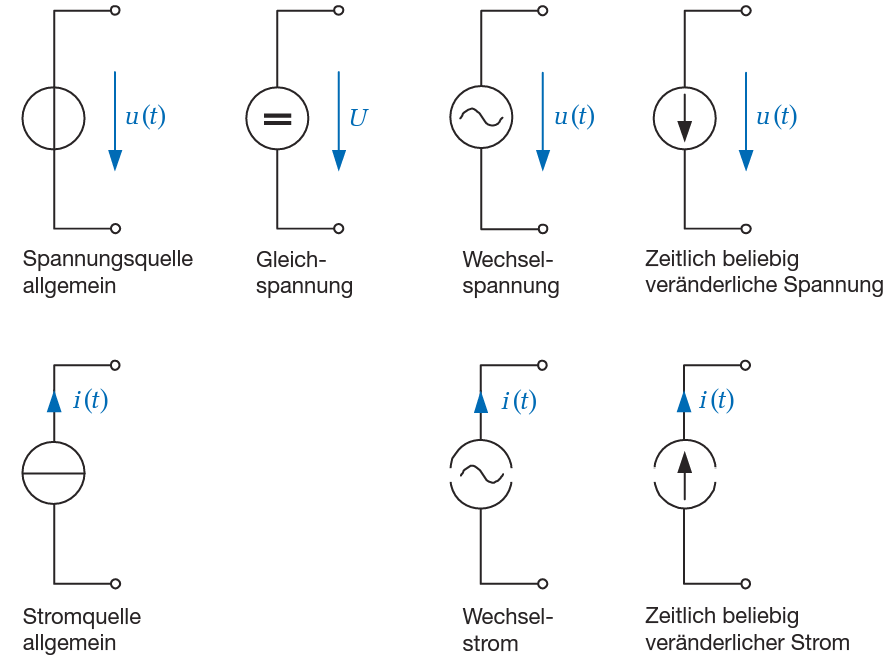
\includegraphics[scale=0.65]{../img/IIId}}
\centering
\caption{Ideale Spannungs- und Stromquellen.}
\label{fig_IIId}
\end{figure}
\subsection{Elemente von Stromkreisen}
Zur Darstellung von Stromkreisen oder Netzwerken werden Symbole, Schaltzeichen und Konvenktionen benützt. Folgende Eintore bzw. Bauelemente werden verwendet: Spannungsquelle $U_q$, Stromquelle $I_q$ und Widerstand $R$. Diese Bauelemente stellen ein idealisiertes Verhalten dar und haben folgende Eigenschaften
\begin{itemize}
\item Die ideale Spannungsquelle liefert eine konstante Spannung bei beliebigem Strom
\item Die ideale Stromquelle liefert einen konstanten Strom bei beliebiger Spannung
\item Der Widerstand ist linear und konstant
\end{itemize}
Werden die verwendeten Schaltzeichen (Eintore) mit Zählpfeilen versehen, so kann wahlweise mit dem VZS oder EZS gearbeitet werden. Besitzt ein Netzwerk Eingangsklemmen und Ausgangsklemmen, so bezeichnet man dieses als Zweitor.
\newline\newline
Ein- und Zweitore werden eingeteilt in \textbf{passive}, \textbf{verlustlose} und \textbf{aktive} Ein- und Zweitore. Dabei muss noch zwischen aktivem $n$-Tor und \textbf{aktiv wirkenden} $n$-Tor unterschieden werden. Ein- und Zweitore können in verschiedenen \textbf{Betriebszuständen} betrieben werden. So kann ein aktives Eintor auch einen Betriebszustand aufweisen, wo es passiv wirkt, also Leistung aufnimmt.
\newline\newline
\textbf{Passiver Betriebszustand: } Das $n$-Tor nimmt in diesdem Betriebszustand mehr Leistung auf wie es abgibt.
\newline\newline
\textbf{Verlustloser Betriebszustand: } Das $n$-Tor nimmt in diesdem Betriebszustand gleichviel Leistung auf wie es abgibt.
\newline\newline
\textbf{Aktiver Betriebszustand: } Das $n$-Tor nimmt in diesdem Betriebszustand mehr Leistung ab wie es aufnimmt.
\begin{table}[H]
\centering
\begin{tabular}{lllll}
\hline
&Passiv&Verlustlos&Aktiv&Kommentar\\\hline
Passives $n$-Tor&Normal&Möglich&Nicht möglich&keine Quellen\\
Verlustloses $n$-Tor&Nicht&Normal&Nicht möglich&nur verlustlose Elemente\\
Aktives $n$-Tor&Möglich&Möglich&Möglich&muss Quellen haben\\
\hline
\end{tabular}
\caption{Allgemeines $n$-Tor aufverschiedene Betriebszustände}
\end{table}
\noindent Ein eletrisches Netzwerk aus Eintore und Zweitore wird auf der Ebene projiziert bzw. dargestellt. Die Schaltung enthält die eben eingeführten Schaltzeichen, die idealisierte Bauelemente verkörpern.
\newline\newline
Die einzelne Elemente sind durch \textbf{Linien} miteinander verbunden. Diese Verbin-dungslinien sind widerstandslos und ohne jede andere Wirkung des elektrischen Stromes anzusehen.
\newline\newline
In den \textbf{Knoten} sollen mindestens 3 Verbindungsleitungen zusammentreffen. Ein \textbf{Zweig} verbindet zwei Knoten
\newline\newline
Unter einer \textbf{Masche} versteht man einen in sich geschlossenen Kettenzug bzw. Ringschaltung von Zweigen und Knoten. Geht man von irgend einem Knoten aus, so durchwandert man eine Masche, wenn man, ohne irgend einen Zweig mehrfach zu durchlaufen, zum Ausgangspunkt zurückkehrt.
\subsection{Zählpfeilsysteme}
Ein Zählpfeilsystem am ohmschen Widerstand bei dem Strom und Spannung gleich gerichtet sind heisst \textbf{Verbraucherzählpfeilsystem}. Für $U>0$ wird der in die positive Anschlussklemme hineinfliessende Strom positiv gezählt.
\begin{figure}[H]
\frame{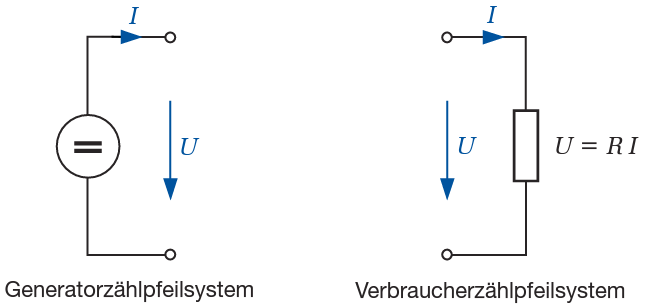
\includegraphics[scale=0.75]{../img/IIIe}}
\centering
\caption{Generator- und Verbraucherzählpfeilsystem.}
\label{fig_IIIe}
\end{figure}
\noindent Für die Quellen verwendet man üblichwerweise das \textbf{Generatorzählpfeilsystem}, bei dem Spannung und Strom entgegengesetzt gerichtet sind. Der aus der positiven Anschlussklemme herausfliessende Strom wird positiv gezählt. Diese Festlegung ist angepasst an den physikalischen Hintergrund, dass der Generator (Quelle) die Energie liefert, während der Verbraucher die Energie aufnimmt.
\subsection{Das ohmsche Gesetz}
In einem linearen Leiter sind Strom und Spannung zueinander proportional. Bei einem linearen Leiter ist der ihn durchfliessenden Strom der angelegten Spannung proportional und dem Leiterwiderstand gegenüber umgekehrt proportional.
\begin{equation}
\boxed{I\left(U\right)=\dfrac{U}{R}=U\cdot G}
\end{equation}
Das \textbf{ohmsche Gesetz} ist ein Grundgesetz des elektrischen Stromes in Leitern. Als ohmschen Widerstand bezeichnet man einen idealen Zweipol, bei dem das ohmsche Gesetz unabhängig von äusseren Einflüssen stets erfüllt ist. Ein ohmscher Widerstand ist ein linearer passiver Zweipol: seine $I$-$U$-Kennlinie ist eine Gerade.
\subsection{Die Kirchhoffschen Gesetze}
Eine der Hauptaufgaben der \textbf{Netzwerkanalyse} besteht darin, die Ströme und Spannungen an den einzelnen Zweipolen auszurechnen, sofern die verwendeten Netzwerkelemente (Widerstände, Kondensatoren, usw), ihre Verknüpfungen untereinander sowie die Quellen innerhalb des Netzwerkes bekannt sind.
\newline\newline
Die schwarz ausgefüllten Markierungspunkte oder \textbf{Knoten} in dem Netzwerk zeigen an, dass die Leitungen an dieser Stelle elektrisch leitend miteinander verbunden sind, z.B. durch Zusammenschrauben oder Verlöten. Die Kreisringe markieren diejenigen Punkte im Netzwerk, zwischen denen die eingezeichnete Spannung gemessen wird.
\begin{figure}[H]
\frame{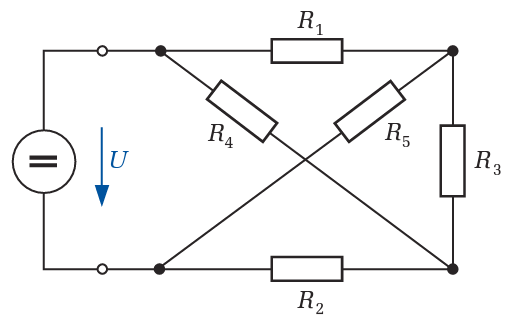
\includegraphics[scale=0.5]{../img/IIIf}}
\frame{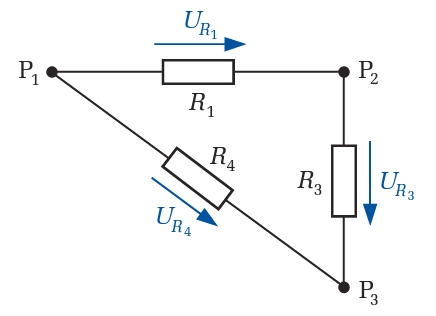
\includegraphics[scale=0.5]{../img/IIIg}}
\frame{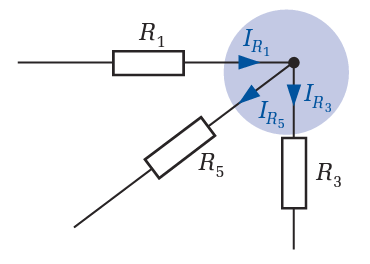
\includegraphics[scale=0.5]{../img/IIIh}}
\centering
\caption{Einfaches Netzwerk, Maschen- und Knotenregel.}
\label{fig_IIIf}
\end{figure}
\noindent Zur allgemeinen Netzwerkanalyse werden offenbar weitere Bestimmungsgleichungen benötigt. Einen ersten Zusammenhang erhält man aus dem Umlaufintegral der elektrischen Feldstärke, welches entlang eines geschlossenen Weges verschwinden muss. Zur Verdeutlichung dieses Zusammenhangs betrachtet man eine \textbf{Masche} in dargestellten Netzwerk.
\newline\newline
\textbf{Knotensatz:} In jedem Knoten (auch Superknoten) ist die Summe der zufliessenden Ströme gleich der Summe der abfliessenden Ströme.
\begin{equation}
\boxed{\displaystyle \sum_{k=1}^nI_k=0}
\end{equation}
\textbf{Maschensatz:} Wird in einem Potentialfeld eine Ladung vom Ausgangspunkt $A$ aus bewegt und wieder zurück zum Punkt $A$ gebracht, so ist die verrichtete Arbeit Null und somit ist auch die Spannung Null. In jeder Masche ist die Summe aller Spannungen (Umlaufspannung) gleich Null.
\begin{equation}
\boxed{\displaystyle \sum_{k=1}^nU_k=0}
\end{equation}
Die Bezugspfeile für alle Spannungen sind entsprechend dem Umlaufsinn zu orientieren. Wenn der Bezugssinn einer Spannung nicht mit dem Umlaufsinn übereinstimmt, wird beim Aufstellen der Maschengleichung diese Spannung mit dem entsprechenden Vorzeichen versehen.
\newline\newline
Im Beispiel lauten die Gleichungen
\begin{equation}
\begin{array}{lll}
I_{R_1}-I_{R_3}-I_{R_5}&=&0\\
I_{R_3}+I_{R_4}-I_{R_2}&=&0\\
U_{R_1}+U_{R_3}-U_{R_4}&=&0\\
U_{R_3}+U_{R_2}-U_{R_5}&=&0\\
U_{R_1}+U_{R_3}+U_{R_2}-U&=&0
\end{array}
\end{equation}
\newline\newline
Ohmsches Gesetz, Knotensatz und Maschensatz sind drei grundlegende Gesetze, mit denen schon allgemeine Netzwerkprobleme gelöst werden können.
\subsection{Leistung und Arbeit}
Wird ein Leiter an eine Gleichspannung $U$ angeschlossen, so fliesst durch ihn ein Strom $I$. Ist $Q$ dabei die durch den Leiterquerschnitt hindurchtretende Ladung, so ist zum Überwinden des Leiterwiderstandes $R$ die \textbf{Energie} $W=Q\cdot U$ erforderlich, es muss also die Arbeit $W$ geleistet werden, um den Strom $I$ durch den Leiter aufrecht zu erhalten.
\newline\newline
Die Energie $W$ mit Einheit $\left([W]=\text{W}\,\text{s}=\text{J}=\text{N}\,\text{m}\right)$ muss von der speisenden Quelle als Energiequelle aufgebracht werden. Praktisch interessiert wie schnell diese Arbeit geleistet werden muss, das ist die Leistungsaufnahme $P$ mit Einheit $\left([P]=\text{W}\right)$ des betrachteten Leiters vom Widerstand $R$.
\begin{equation}
\boxed{P=\dfrac{W}{t}=\dfrac{Q\cdot U}{t}=\dfrac{U\cdot I\cdot \bcancel{t}}{\bcancel{t}}=U\cdot I=I^2\cdot R=\dfrac{U^2}{R}}
\end{equation}
Die in einem Widerstand verbrauchte Energie wird restlos in Wärme umgewandelt. Ein elektrischer Widerstand ist demnach ein Energiewandler, der elektrische Energie in \textbf{Wärme} oder \textbf{mechanische Energie} umwandelt.
\newline\newline
Die nutzbare abgegebene Leistung $P_{\text{ab}}$ ist um die Verlustleistung $P_{\text{verl}}$ kleiner als die zugeführte Leistung $P_{\text{zu}}$. Anstelle der Verluste wird häufig der \textbf{Wirkungsgrad} $\eta$ eines Gerätes angegeben
\begin{equation}
\boxed{P_{\text{zu}}=P_{\text{ab}}+P_{\text{Verl}}}\quad \boxed{\eta=\dfrac{P_{\text{ab}}}{P_{\text{zu}}}\leq 1}
\end{equation}
\subsection{Einfache Schaltungen von Widerständen}
Die Netzwerkanylsse kann dadurch vereinfacht werden, dass einzelne Teile eines Betzwerks vorab zusammengefasst werden. Dabei muss lediglich darauf geachtet werden, dass sich das Klemmenverhalten des neuen vereinfachten Netzwerks gegenüber dem ursprünglichen Netzwerk nicht ändert, d.h. beim Anlegen der gleichen Spannung an die Klemmen muss in beiden Fällen der gleiche Strom fliessen.
\newline\newline
Mit Hilfe von Knotensatz, Maschensatz und ohmsches Gesetz können nun für die Serienschaltung und Parallelschaltung von Widerständen einfache Regeln hergeleitet werden.
\subsection{Reihenschaltung - Spannungsteiler}
\begin{figure}[H]
\frame{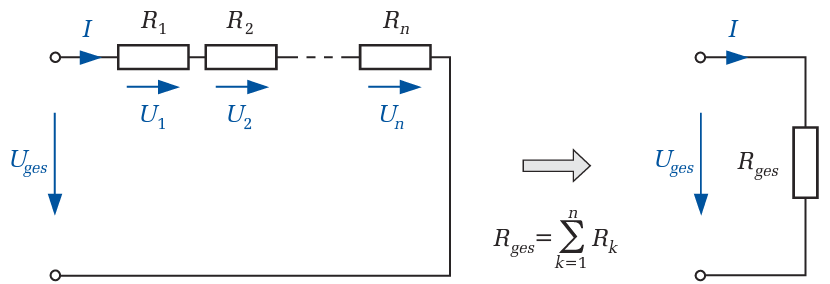
\includegraphics[scale=0.75]{../img/IIIk}}
\centering
\caption{Reihenschaltung von $n$ Widerständen.}
\label{fig_IIIk}
\end{figure}
Bei einer \textbf{Reihenschaltung} werden alle Widerstände von dem gleichen Strom $I$ durchfliessen. Die gesamte anliegende Spannung $U_{\text{ges}}$ entsprechend dem Maschenumlauf setzt sich aus den Teilspannungen $U_k$ an den einzelnen Widerständen $R_k$ zusammen.
\newline\newline
Bei der Reihenschaltung von Widerstände, addieren sich die Werte der einzelnen Widerstände und der Gesamtwiderstand ist grösser als der grösste Einzelwiderstand.
\begin{equation}
\boxed{U_{\text{ges}}=\displaystyle \sum_{k=1}^nU_k=\displaystyle \sum_{k=1}^n\left(R_k\cdot I\right)=\underbrace{\left(\displaystyle \sum_{k=1}^nR_k\right)}_{R_{\text{ges}}}\cdot I}\quad \boxed{R_{\text{ges}}=\displaystyle \sum_{k=1}^nR_k}
\end{equation}
Fliesst der gleiche Strom durch mehrere in Reihe geschaltete Widerstände, dann stehen die Teilspannungen im gleichen Verhältnis wie die Teilwiderstände, an denen sie abfallen.
\begin{equation}
\boxed{\dfrac{U_i}{U_{i+1}}=\dfrac{R_i}{R_{i+1}}}\quad \boxed{\dfrac{U_i}{U_{\text{ges}}}=\dfrac{U_i}{\displaystyle \sum_{k=1}^n U_k}=\dfrac{\bcancel{I}\cdot R_i}{\bcancel{I}\cdot \displaystyle \sum_{k=1}^n R_k}=\dfrac{R_i}{R_{\text{ges}}}}
\end{equation}
Infolge des gleichen Stromes stehen die \textbf{Leistungen} an den Widerständen im gleichen Verhältnis zueinander wie die Spannungen und wie die Widerstände. Die an einem Widerstand entstehende Teilspannung wird als \textbf{Spannungsabfall} bezeichnet.
\newline\newline
Definiert man das Potential am Minusanschluss der Spannungsquelle als Bezugswert $V=0$, dann besitzt das Potential am positiven Anschluss den Wert $V=U$. Mit einem ortsunabhängigen Feldstärkeverlauf innerhalb der Widerstände nimmt das Potential linear ab und man erhält entlang der Reihenschaltung für ein angenommenes Widerstandsverhältnis dargestellten Potentialverlauf.
\subsubsection{Beispiel einer Reihenschaltung}
\begin{figure}[H]
\frame{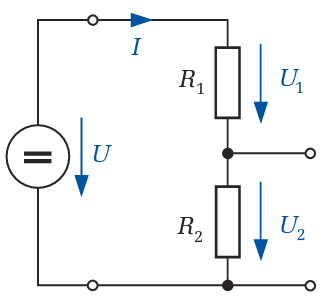
\includegraphics[scale=0.65]{../img/IIIm}}\quad
\frame{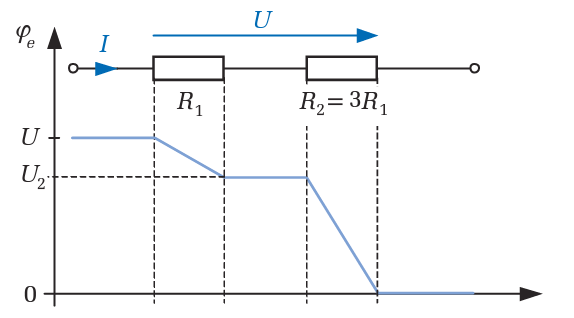
\includegraphics[scale=0.65]{../img/IIIn}}
\centering
\caption{Schaltung zur Spannungsteilung und Potentialverlauf.}
\label{fig_IIIm}
\end{figure}
\textbf{Maschensatz:} $-U+U_1+U_2=0\Longrightarrow U=U_1+U_2$\\
\textbf{Ohmsches Gesetz:} $U_1=R_1\cdot I\quad U_2=R_2\cdot I$\\
\textbf{Verhältnis:} $\dfrac{U_1}{U_2}=\dfrac{R_1\cdot \bcancel{I}}{R_2\cdot \bcancel{I}}$\\
\textbf{Verhältnis:} $\dfrac{U_2}{U}=\dfrac{U_2}{U_1+U_2}=\dfrac{R_2\cdot \bcancel{I}}{\left(R_1+R_2\right)\cdot \bcancel{I}}$
\subsection{Parallelschaltung - Stromteiler}
\begin{figure}[H]
\frame{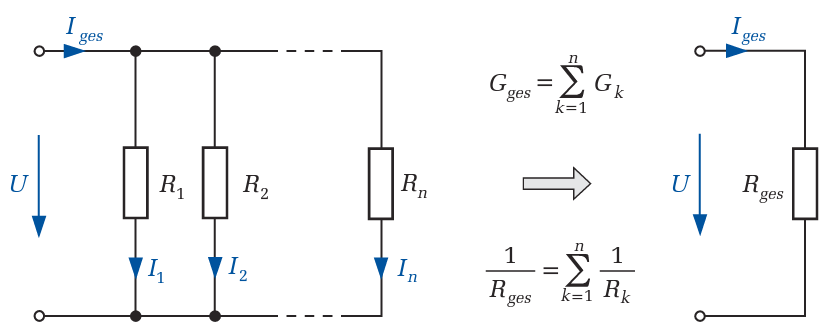
\includegraphics[scale=0.75]{../img/IIIl}}
\centering
\caption{Parallelschaltung von $n$ Widerständen.}
\label{fig_IIIk}
\end{figure}
\noindent Bei der \textbf{Parallelschaltung} ist die Spannung $U$ an allen Widerständen gleich gross und der gesamte Eingangsstrom $I_{\text{ges}}$ setzt sich aus den Teilströmen $I_k$ durch die einzelnen Widerstände $R_k$ zusammen. Bei der Parallelschaltung ist die Verwendung der Leitwerte sinnvoll.
\newline\newline
Bei der Parallelschaltung berechnet sich der gesamte Leitwert aus der Summe der einzelnen Leitwerte und der Gesamtwiderstand ist kleiner als der kleinste Einzelwiderstand.
\begin{equation}
\boxed{I_{\text{ges}}=\displaystyle \sum_{k=1}^nI_k=\displaystyle \sum_{k=1}^n\left(\dfrac{U}{R_k}\right)=U\cdot \underbrace{\left(\displaystyle \sum_{k=1}^n\dfrac{1}{R_k}\right)}_{G_{\text{ges}}}}\quad \boxed{R_{\text{ges}}=\dfrac{1}{G_{\text{ges}}}=\dfrac{1}{\displaystyle \sum_{k=1}^n\dfrac{1}{R_k}}=\dfrac{\displaystyle \prod_{k=1}^nR_k}{\displaystyle \sum_{k=1}^nR_k}}
\end{equation}
\begin{equation}
\boxed{\dfrac{I_i}{I_{i+1}}=\dfrac{G_i}{G_{i+1}}=\dfrac{R_{i+1}}{R_i}}\quad \boxed{\dfrac{I_i}{I_{\text{ges}}}=\dfrac{I_i}{\displaystyle \sum_{k=1}^nI_k}=\dfrac{\bcancel{U_i}\cdot \dfrac{1}{R_i}}{\bcancel{U_i}\cdot \displaystyle \sum_{k=1}^n\dfrac{1}{R_k}}=\dfrac{G_i}{G_{\text{ges}}}}
\end{equation}
\noindent Für den Sondernfall mit nur zwei parallel geschalteten Widerständen gilt
\begin{equation}
\boxed{R_{\text{ges}}=\dfrac{R_1\cdot R_2}{R_1+R_2}}
\end{equation}
Für den Sondernfall mit $n$ parallel gleiche geschalteten Widerständen gilt
\begin{equation}
\boxed{R_{\text{ges}}=\dfrac{R}{n}}
\end{equation}
Liegt die gleiche Spannung an mehreren parallel geschachtelten Widerständen, dann stehen die Ströme im gleichen Verhältnis wie die Leitwerte, die sie durchfliessen. Die \textbf{Leistungen} an den Widerständen verhalten sich wegen der gleichen Spannung wie die Ströme durch die Widerstände und stehen im gleichen Verhältnis wie die Leitwerte.
\subsubsection{Beispiel einer Parallelschaltung}
\begin{figure}[H]
\frame{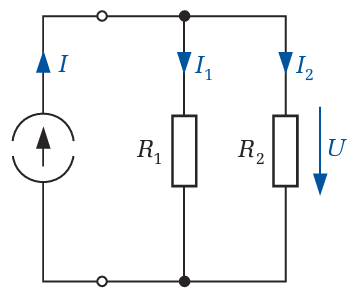
\includegraphics[scale=0.75]{../img/IIIr}}
\centering
\caption{Schaltung zur Stromleitung.}
\label{fig_IIIr}
\end{figure}
\textbf{Knotensatz:} $-I+I_1+I_2=0\Longrightarrow I=I_1+I_2$\\
\textbf{Ohmsches Gesetz:} $I_1=\dfrac{U}{R_1}\quad I_2=\dfrac{U}{R_2}$\\
\textbf{Verhältnis:} $\dfrac{I_1}{I_2}=\dfrac{R_2}{R_1}=\dfrac{G_1}{G_2}$\\
\textbf{Verhältnis:} $\dfrac{I_2}{I}=\dfrac{R_1}{R_1+R_2}=\dfrac{G_2}{G_1+G_2}$
\begin{comment}
\subsection{Serieschaltung von Widerständen - Spannungsteilung}
Anwendung des Maschensatzes und des ohmsches Gesetzes liefert in einer Serienschaltung
\begin{equation}
\boxed{\displaystyle \sum_{k=1}^nU_k-U_q=\displaystyle \sum_{k=1}^nI\cdot R_k-U_q=I\cdot \underbrace{\displaystyle \sum_{k=1}^nR_k}_{R_E}-U_q=0\Longrightarrow U_q=I\cdot R_E}
\end{equation}
Damit ergibt sich für den \textbf{Ersatzwiderstand} $R_E$ und für das Verhältnis jeder Spannung zum Spannungsquelle die folgende \textbf{Spannungsteilung}
\begin{equation}
\boxed{R_E=\displaystyle \sum_{k=1}^nR_k}\quad \boxed{\dfrac{U_k}{U_q}=\dfrac{I\cdot R_k}{I\cdot R_E}=\dfrac{R_k}{R_E}}
\end{equation}
Bei in Serie geschalteten Widerständen ist der Ersatzwiderstand die Summe der einzelnen Widerstände. Bei in Serie geschalteten Widerständen teilt sich die Spannung direkt proportional zu jedem Widerstand.
\subsection{Parallelschaltung von Widerständen - Stromteilung}
Anwendung des Knotensatzes und des ohmschen Gesetzes liefert in einer Parallelschaltung
\begin{equation}
\boxed{\displaystyle \sum_{k=1}^n I_k-I_q=\displaystyle \sum_{k=1}^n \dfrac{U}{R_k}-I_q=U\cdot \underbrace{\displaystyle \sum_{k=1}^n \dfrac{1}{R_k}}_{G_E}-I_q=0\Longrightarrow I_q=U\cdot G_E}
\end{equation}
Damit ergibt sich für den \textbf{Ersatzleitwert} $G_E$ und für das Verhältnis jedem Strom zum Stromquelle die folgende \textbf{Stromteilung}
\begin{equation}
\boxed{G_E=\displaystyle \sum_{k=1}^n\dfrac{1}{R_k}}\quad \boxed{\dfrac{I_k}{I_q}=\dfrac{U\cdot G_k}{U\cdot G_E}=\dfrac{G_k}{G_E}=\dfrac{R_E}{R_k}}
\end{equation}
Bei parallel geschalteten Widerständen ist der Ersatzleitwert die Summe der einzelnen Leitwerte. Bei parallel geschalteten Widerständen teilt sich der Strom direkt proportional zu den Leitwerten bzw. indirekt proportional zu jedem Widerstand.
\end{comment}
\subsection{Anwendungen der Schaltungen}
\subsubsection{Der belastete Spannungsteiler}
\begin{figure}[H]
\frame{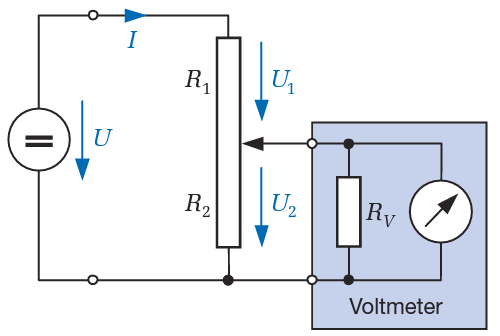
\includegraphics[scale=0.65]{../img/IIIo}}
\frame{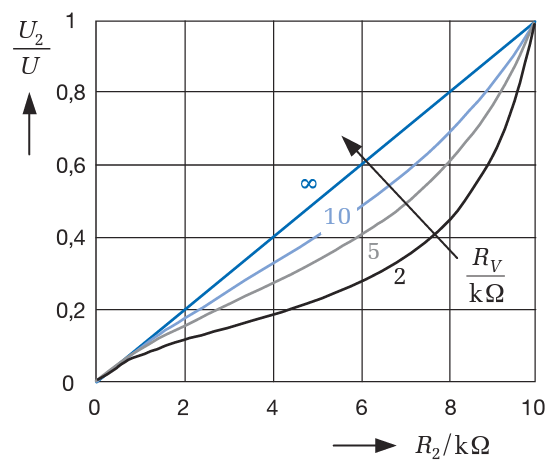
\includegraphics[scale=0.55]{../img/IIIp}}
\centering
\caption{\textbf{\textit{Links:}} Belasteter Spannungsteiler. \textbf{\textit{Rechts:}} Ausgangsspannung am belasteten Spannungsteiler für $R_1+R_2=10k\Omega$}
\label{fig_IIIo}
\end{figure}
\noindent Die Spannung an dem Schleifkontakt eines Potentiometers soll mit einem realen \textbf{Spannungsmessgerät} (Voltmeter) gemessen werden. Dabei ist zu beachten, dass fast alle Spannungsmessgeräte von einem kleinen Strom durchflossen werden, der die in \textbf{Gleichung des Spannungsteilers} berechnete Spannungsteilung beeinflusst und das Messergebnis verfälscht. Diese Einfluss kann man erfassen, indem man das reale Messgerät durch ein ideales Messgerät mit unendlich grossem Innenwiderstand und zusätzlich durch einen parallel geschalteten Widerstand $R_V$ ersetzen.
\noindent Die Berechnung der resultierenden Spannung $U_2$ wird wesentlich vereinfacht, wenn man die Parallelschaltung der beiden WIderstände $R_2$ und $R_V$ durch einen neuen Widerstand $R_{\text{par}}$ ersetzen und die Spannung $U_2$ aus der Reihenschaltung von $R_1$ und $R_{\text{par}}$ bestimmen.
\begin{equation}
\boxed{R_{\text{par}}=\dfrac{R_2\cdot R_V}{R_2+R_V}}\quad \boxed{\dfrac{U_2}{U}=\dfrac{R_{\text{par}}}{R_1+R_{\text{par}}}}
\end{equation}
\subsubsection{Messbereich eines Spannungsmessgerätes}
\begin{figure}[H]
\frame{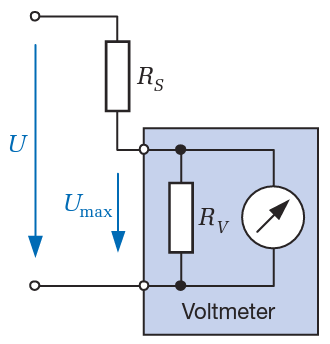
\includegraphics[scale=0.65]{../img/IIIq}}
\centering
\caption{Voltmeter mit Vorwiderstand.}
\label{fig_IIIs}
\end{figure}
\noindent Ein Anwendungsbeispiel für den Spannungsteiler ist die Messbereichserweiterung eines Voltmeters. Soll mit dem Messgerät eine Spannung $U$ gemessen werden, die die maximal zulässige Spannung am Voltmeter $U_{\text{max}}$ überschreitet, dann kann die zu messende Spannung mit einem in Serie geschalteten Vorwiderstand $R_S$ heruntergeteilt weerden. Der Wert des Vorwiderstandes kann mit Hilfe der \textbf{Gleichung des Spannungsteilers} berechnet werden.
\begin{equation}
\boxed{\dfrac{U_{\text{max}}}{U}=\dfrac{R_V}{R_S+R_V}}
\end{equation}
\subsubsection{Messbereich eines Strommessgeräts}
\begin{figure}[H]
\frame{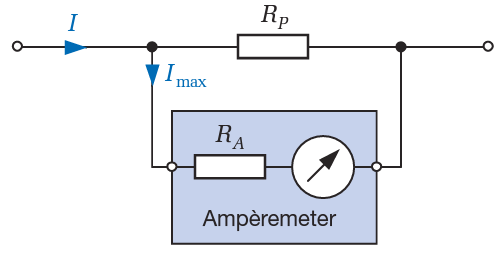
\includegraphics[scale=0.65]{../img/IIIs}}
\centering
\caption{Ampèremeter mit Parallelwiderstand.}
\label{fig_IIIs}
\end{figure}
\noindent Zur Messung eines Stromes wird das \textbf{Ampèremeter} in den Strompfad geschaltet, sein Innenwiderstand  $R_A$ sollte daher möglichst gering sein, um das Messergebnis nur wenig zu beeinflussen. Soll ein Strom gemessen werden, der den maximal zulässigen Bereich des Ampèremeters $I_{\text{max}}$ überschreitet, dann kann der Gesamtstrom $I$ durch einen parallel geschalteten Widerstand heruntergeteilt werden. Der Wert des Parallelwiderstandes kann mit Hilf der \textbf{Gleichung des Stromleiters} berechnet werden.
\begin{equation}
\boxed{\dfrac{I_{\text{max}}}{I}=\dfrac{R_P}{R_P+R_A}}
\end{equation}
\subsubsection{Widerstandsmessung}
\begin{figure}[H]
\frame{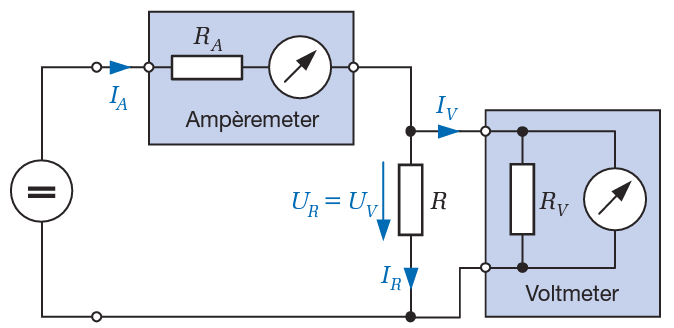
\includegraphics[scale=0.65]{../img/IIIt}}
\centering
\caption{Korrekte Spannungsmessung.}
\label{fig_IIIu}
\end{figure}
Bei der obigen Schaltung wird die Spannung am Widerstand richtig erfasst, dass Ampèremeter misst allerdings nicht nur den Strom $I_R$ durch den Widerstand, sondern zusätzlich auch noch den Strom $I_V$ durch das Voltmerer. Für den Widerstandswert $R$ erhält man
\begin{equation}
\boxed{R=\dfrac{U_R}{I_R}=\dfrac{U_V}{I_A-I_V}=\dfrac{U_V}{I_A-U_V/R_V}=\dfrac{U_VR_V}{I_AR_V-U_V}}
\end{equation}
Der Innenwiderstand des Ampèremeters spielt bei dieser Messanordnung keine Rolle. Im Falle eines idealen Voltmeters $R_V\rightarrow \infty$ vereinfacht sich die obige Gleichung auf den Zusammenhang $R=U_V/I_A$, d.h. der Wert $R$ kann direkt aus den beiden Messwerten berechnet werden.
\begin{figure}[H]
\frame{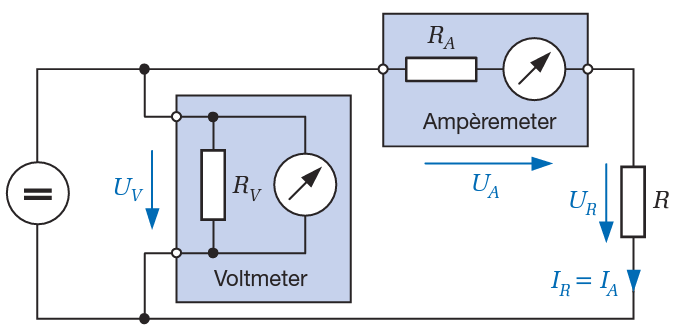
\includegraphics[scale=0.65]{../img/IIIu}}
\centering
\caption{Korrekte Spannungsmessung.}
\label{fig_IIIu}
\end{figure}
\noindent Bei den alternativen Messanordnung wird der Strom durch den Widerstand richtig gemessen, allerdings wird jetzt der Spannungsabfall $U_A$ am Innenwiderstand des Ampèremeters bei der Spannungsmessung miterfasst. Den Widerstandswert erhält man aus der Bezeichnung
\begin{equation}
\boxed{R=\dfrac{U_R}{I_R}=\dfrac{U_V-U_A}{I_A}=\dfrac{U_V-R_AI_A}{I_A}}
\end{equation}
In diesem Fall spielt der Innenwiderstand des Voltmeters keine Rolle. Im Falle eines idealen Ampèremeters $R_A\rightarrow 0$ vereinfacht sich die obige Gleichung auf den Zusammenhang $R=U_V/I_A$, d.h. der Wert $R$ kann wieder direkt aus den beiden Messwerten berechnet werden.
\newline\newline
Allgemein stellt man sich die Aufgabe, den ohmschen Widerstand $R$ eines Bauteils durch gleichzeitige Strom- und Spannungsmessung und mit Hilfe des Ohm'-schen Gesetzes zu bestimmen. Da das Ampèremeter den Strom durch den Widerstand messen soll, muss es in Reihe zum Widerstand geschaltet werden. Zur Erfassung der Spannung am Widerstand muss das Voltmeter aber parallel zum Widerstand angeschlossen werden.



\subsection{Quellen, Ersatzschaltungen und Kennlinien}
Man betrachte ein beliebiges Netzwerk aus Widerständen, Spannungs- und Stromquellen besteht. Nun wird das Netzwerk an zwei Klemmen zugänglich gemacht. Belastet man jetzt das Netzwerk, so sind $U_a$ und $I_a$ linear voneinander abhängig (Gerade in $U$-$I$-Kennlinie).
\newline\newline
Die lineare Abhängigkeit zwischen $U_a$ und $I_a$ kann in der Form $U_a=\alpha\cdot I_B+\beta$ geschrieben werden. Die Parameter $\alpha$ und $\beta$ sind unabhängig von der Belastung sondern vom gegebenen Netzwerk abhängig.
\newline\newline
Das gegebene Netzwerk soll in seinem Innern durch ein möglichst einfaches Ersatznetzwerk ersetzt werden, so dass die Wirkung nach aussen an den Klemmen unverändert bleiben. Ein äusserer Beobachter kann nicht festlegen, dass im Innern das komplizierten Netzwerk durch ein einfacheres Netzwerk ausgetauscht wurde.
\newline\newline
Die Ersatznetzwerke sind die \textbf{Thevenin'sche Ersatzschaltung} (eine ideale Spannungsquelle mit Seriewiderstand) und die \textbf{Norton'sche Ersatzschaltung} (eine ideale Stromquelle mit Parallelwiderstand) unter der Bedingung, dass der Ersatz bezüglich zweier wohldefinierter Klemmen geschieht. Das Ersatznetzwerk weist die gleiche Wirkung wie das Originalnetzwerk auf. Beide Ersatzschaltungen sind mit zwei Grössen vollständig beschrieben und daher lässt sich die $U_a$-$I_a$-Gerade nachbilden.
\newline\newline
Die zwei Grössen $U_{qe}$ und $R_{qe}$ bzw. $I_{qe}$ und $R_{qe}$ der Ersatzschaltungen sind nun mit geeigneten Überlegungen und Experimenten an den Klemmen zu bestimmen.
\newline\newline
Zwei beliebige Punkte auf der $U_a$-$I_a$-Geraden genügen, um die Ersatzschaltungen nach Thevenin oder Norton vollständig zu beschreiben. Lässt man die Klemmen $1$-$1'$ offen (Leerlauf), so misst man an ihnen die sogenannte \textbf{Leerlaufspannung} $U_{\text{LL}}$, schliesst man die Klemmen kurz, so fliesst der sogenannte \textbf{Kurzschlussstrom} $I_{\text{KS}}$. Diese zwei Punkte sind extreme Betriebszustände. Schaltet man alle inneren Quellen ab, so wird das Netzwerk passiv, d.h. seine Kennlinie verläuft nun durch den Nullpunkt.
\newline\newline
Abschalten einer Quelle bedeutet, sie durch ihren Innenwiderstand zu ersetzen. Bei der idealen Spannungsquelle ist der Innenwiderstand Null $U_q=0$. Für die ideale Stromquelle ist der Innenwiderstand unendlich $I_q=0$.
\newline\newline
Die $U_a$-$I_a$-Kennlinie des passiven Netzwerkes durch den Nullpunkt entspricht der Kennlinie eines ohmschen Widerstandes. Dieser ohmsche Widerstand ist der \textbf{Ersatzwiderstand}, wenn bei \textbf{abgeschalteten Quellen} bei den Klemmen $1$-$1'$ in das Netzwerk hineingemessen wird. Dieser gemessene Widerstand wird dann gerade zum Widerstand $R_e$ der Ersatzschaltung nach Thevenin oder nach Norton.
\newline\newline
Beim Abschalten einer Quelle wird sie nicht einfach weggelassen, sondern durch ihren Innenwiderstand ersetzt. Beim Abschalten einer Quelle wird die ideale Spannungsquelle durch einen Kurzschluss und die ideale Stromquelle durch einen Unterbruch ersetzt.
\newline\newline
Damit stehen nun drei Experimente zur Verfügung, um die zwei Grössen $U_{qe}$ und $R_{qe}$ bzw. $I_{qe}$ und $R_{qe}$ der Ersatzschaltung zu bestimmen.
\newline\newline
Von obigen drei Experimenten genügen zwei um die Ersatzschaltung zu bestimmen. Die drei Grössen $U_{qe}$, $I_{qe}$ und $R_{qe}$ sind voneinander abhängig.
\begin{equation}
\boxed{U_{qe}=R_{qe}\cdot I_{qe}}
\end{equation}
Die beiden Ersatzschaltungen nach Thevenin und Norton sind vollständig gleichwertig. Mit obiger Gleichung kann eine Thevenin-Ersatzschaltung in einer Norton-Erschatzschaltung umgewandelt werden und umgekehrt.
\newline\newline
Belastet eine Quelle (Ersatzschaltung eines linearen Netzwerkes) mit einem variablen Lastwiderstand, sowerden folgende Bezeichnungen eingeführt: $U_{qe}$ ist die Leerlaufspannung, $R_{qe}$ ist der Innenwiderstand bzw. der Ersatzwiderstand, $R_L$ ist der Lastwiderstand, $U_a$ zwischen $1$-$1'$ ist die Klemmenspannung und $I_a$ der Klemmestrom.
\newline\newline
Fasst man $I_a$ als unabhängige und $U_a$ als abhängige Variable auf, so bezeichnet man die Funktion $U_a=f\left(I_a\right)$ und ihre graphische Darstellung als \textbf{Quellenkennlinie}. Die Schnittpunkte mit den Achsen sind der Leerlauf mit $U_{\text{LL}}=U_{qe}$ und der Kurzschluss $I_{\text{KS}}$.
\begin{equation}
\boxed{U_a=U_{qe}-I_a\cdot R_{qe}}
\end{equation}
\begin{equation}
\boxed{I_{\text{KS}}=\dfrac{U_{qe}}{R_{qe}}}\quad \boxed{R_{qe}=-\dfrac{\triangle U_a}{\triangle I_a}}
\end{equation}
Führt man für Quelle und Lastwiderstand je eine Kennlinie ein, so werden beim Zusammenschalten von Quelle und Lastwiderstand die beiden Kennlinien in ein gemeinsames Koordinatensystem gezeichnet. Den Schnittpunkt der beiden Kennlinien bezeichnet man als \textbf{Arbeitspunkt} (AP). Dieser Arbeitspunkt stellt sich dort ein, wo $U_{a1}=U_{a2}$ wird.
\newline\newline
Gleichsetzen von $U_{a1}$ und $U_{a2}$ liefert Strom und Spannung des Arbeitspunktes
\begin{equation}
\boxed{I_{\text{AP}}=\dfrac{U_{qe}}{R_{qe}+R_L}}\quad \boxed{U_{\text{AP}}=\dfrac{U_{qe}\cdot R_L}{R_{qe}+R_L}}
\end{equation}
\subsection{Zusammenschalten von Quellen}
Die Thevenin-Ersatzschaltung einer Quelle wird als ``Thevenin-Quelle'' bezeichnet, ebenso heisst nun die Norton-Ersatzschaltung ener Quelle ``Norton-Quelle''. Werden reale Quellen zusammengeschaltet, so bestimmt man mit den bekannten Methoden das Ersatznetzwerk (Thevenin oder Norton). Werden ideale Quellen parallel ode rin Serie geschaltet, so sind folgende sechs Fälle zu unterscheiden:
\begin{equation}
\boxed{
    \begin{array}{llll}
    \text{U-Quelle}&\text{parallel}&\text{U-Quelle}&\Rightarrow \text{Widerspruch}\\
    \text{U-Quelle}&\text{in Serie}&\text{U-Quelle}&\Rightarrow \text{Addition der Spannungen}\\
    \text{I-Quelle}&\text{in Serie}&\text{I-Quelle}&\Rightarrow \text{Widerspruch}\\
    \text{I-Quelle}&\text{parallel}&\text{I-Quelle}&\Rightarrow \text{Addition der Ströme}\\
    \text{I-Quelle}&\text{parallel}&\text{U-Quelle}&\Rightarrow \text{U-Quelle}\\
    \text{I-Quelle}&\text{in Serie}&\text{U-Quelle}&\Rightarrow \text{I-Quelle}\\
    \end{array}
}
\end{equation}
\subsection{Verfügbare Quellenleistung und Leistungsanpassung}
Eine Quelle wird mit einem variablen Lastwiderstand $R_L$ belastet. Nun wird die an die Last abgegebene Leistung $P_L$ berechnet.
\begin{equation}
\boxed{I=\dfrac{U_q}{R_q+R_L}}\quad \boxed{P_L=I^2\cdot R_L=\dfrac{U_q^2\cdot R_L}{\left(R_q+R_L\right)^2}=f\left(R_L\right)}
\end{equation}
Für $R_L=0$ (Kurzschluss) und $R_L=\infty$ (Leerlauf) wird $P_L=0$. Dazwischen weist $P_L=f\left(R_L\right)$ ein Maximum auf. Mit Nullsetzen der Ableitung von $f\left(R_L\right)$ erhält man den Lastwiderstand für die maximale Leistung
\begin{equation}
\boxed{\dfrac{\text{d}f\left(R_L\right)}{\text{d}R_L}=0\Longrightarrow R_L=R_q}
\end{equation}
Den Betriebszustand mit $R_L=R_q$ bezeichnet man als \textbf{Leistungsanpassung} und eine Quelle gibt ihre verfügbare Leistung an die Last ab. Setzt man $R_L=R_q$ ein,
\begin{equation}
\boxed{P_L=I^2\cdot R_L=\left(\dfrac{U_q}{R_q+R_L}\right)^2\cdot R_L=\left(\dfrac{U_q}{R_q+R_q}\right)^2\cdot R_q}
\end{equation}
so erhält man die maximale Leistung
\begin{equation}
\boxed{P_{L,\text{max}}=P_{\text{AV}}=\dfrac{U_q^2}{4\cdot R_q}}
\end{equation}
Diese Leistung stellt das Maximum dar, welches die Quelle an Leistung abgeben kann. Man bezeichnet sie als \textbf{verfügbare Leistung} (available power). Man beachte, dass $P_{\text{AV}}$ nicht vom Lastwiderstand abhängig ist und jeder Quelle zugeordnet werden kann.
\newline\newline
Das Verhältnis $P_L/P_{\text{AV}}$ in Funktion von $R_L/R_q$ zeigt das Maximum die Leistungsanpassung. Für $R_q=0$ und $R_q=\infty$ ist die verfügbare Leistung nicht definiert.
\begin{equation}
\boxed{\dfrac{P_L}{P_{\text{AV}}}=\dfrac{\dfrac{U_q^2\cdot R_L}{\left(R_q+R_L\right)^2}}{\dfrac{U_q^2}{4\cdot R_q}}=\dfrac{4}{2+\dfrac{R_q}{R_L}+\dfrac{R_L}{R_q}}=\dfrac{4}{2+x+\dfrac{1}{x}}=\dfrac{4}{\left(\sqrt{x}+\dfrac{1}{\sqrt{x}}\right)^2}}
\end{equation}
\section{Analyse von Gleichstromkreisen}
\subsection{Anwendung von Knoten- und Maschensatz}
Mit Hilfe von Knoten- und Maschensatz können Netzwerke gelöst werden. Bei der Anwendung erhält man Gleichungen, die dann mit geeigneten Methoden aufgelöst werden können.
\begin{equation}
\boxed{\displaystyle \sum_{k=1}^nU_k=0}\quad \boxed{\displaystyle \sum_{k=1}^nI_k=0}
\end{equation}
Um Knoten- und Maschensatz aufzustellen, führt man in Netzwerk zusätzliche Ströme ein. Die restlichen Ströme ergeben sich aus den Knotensatz.
\subsection{Netzumwandlung}
Meistens interessiert man sich in einem Netzwerk für eine bestimmte Spannung oder ein bestimmter Strom. Folgende Schritte können durchgeführt werden.
\begin{itemize}
\item Überflüssige Widerstände weglassen oder kurzschliessen.
\item Widerstände bei Serie- oder Parallelschaltungen zusammenfassen.
\item Punkte mit gleichem Potential können getrennt oder verbunden werden.
\item Zusätzliche Einströmungen an Knoten anbringen, ohne Verletzung des Knotensatzes.
\item Teile des Netzwerkes, oder ganzes Netzwerk durch Ersatzquellen ersetzen.
\item Stern-Dreieck-Umwandlung.
\item Weitere Äquivalenztransformationen (LC-Eintore).
\end{itemize}
\subsection{Dreieck-Stern-Umwandlung}
Hier handelt es sich um eine äquivalente Umwandlung eines 3-Pol-Netzwerkes (3 Anschlussklemmen).
\begin{equation}
\boxed{R_A=\dfrac{R_1\cdot R_3}{R_1+R_2+R_3}}\quad \boxed{R_B=\dfrac{R_1\cdot R_2}{R_1+R_2+R_3}}\quad \boxed{R_C=\dfrac{R_2\cdot R_3}{R_1+R_2+R_3}}
\end{equation}
Auch die Rückumwandlung von der Sternschaltung in die Dreiecksschaltung ist möglich. Hier werden Leitwerte statt Widerstände verwendet.
\begin{equation}
\boxed{G_A=\dfrac{G_1\cdot G_2}{G_1+G_2+G_3}}\quad \boxed{G_B=\dfrac{G_2\cdot G_3}{G_1+G_2+G_3}}\quad \boxed{G_C=\dfrac{G_1\cdot G_3}{G_1+G_2+G_3}}
\end{equation}
\subsection{Spannungsquellen verdoppeln}
In einem Netzwerk weisen zwei Punkte mit gleichem Potential gegenüber eines Bezugspunktes auf. Werden nun zwei \textbf{identische Spannungsquellen} an diese Punkte angeschlossen, so kann man die Verbindung zwischen dieser zwei Punkte weglassen. Die Widerstände im Netzwerk haben von dieser Umwandlung nichts bemerkt.
\newline\newline
Jede Spannungsquelle hat nun einen Serienwiderstand und kann in eine \textbf{Norton-Quelle} verwandelt werden, damit lässt sich das Netzwerk weiter vereinfachen.
\subsection{Stromquellen verdoppeln}
Eine Brücke wird mit einer idealen Stromquelle gespeist. Die Stromquelle wird nun verdoppelt und einem Knoten wird der Strom zugeführt und wieder weggeführt. Die Widerstände bemerken nichts von der Umwandlung und die Einströmungsverhältnisse an den Knoten sind unverändert.
\newline\newline
Dank der Umwandlung besitzt jede Stromquelle einen Parallelwiderstand und könnte in eine \textbf{Thevenin-Quelle} verwandelt werden.
\subsection{Ersatzquellen einführen}
Hier handelt es sich um die wirksamste Methode. Ein Strom durch einen Widerstand ist gesucht, alle anderen Spannungen und Ströme sind nicht gefragt. Das Netzwerk wird so weit wie möglich vereinfacht, nur die Verhältnisse beim Widerstand dürfen sich nicht ändern. Der Widerstand wird mit einer Umrandung versehen. Das Netzwerk ausserhalb dieser Umrandung wird jetzt in mehreren Schritten vereinfacht. Im ersten Schritt verdoppelt man die Spannungsquelle.
\newline\newline
Einführen von zwei zusätzliche Klemmen und Umzeichen der Quelle. Blickt man von den Klemmen so kann das linke und das rechte Netzwerk mit einer Ersatzquelle ersetzt werden. Die Ersatzgrössen $U_{{qe}_k}$, $R_{{qe}_k}$, $I_{{qe}_k}$ können bestimmt werden.
\subsection{Überlagerungssatz (Superposition)}
Überlagerung bedeutet, jede Ursache (fliessende Ströme $I_k$, Spannungsquellen $U_k$) wirkt einzeln im Netzwerk. Die Gesamtwirkung erhält man durch Addition der einzelnen Wirkungen. Die Methoden macht nur Sinn, wenn mehrere Quellen beteiligt sind.
\newline\newline
Dabei gelten Konvenktionen: Erster Index ist der Ort, wo der Ursache gemessen wird. Zweiter Index ist der Ort, wo die Ursache wirkt. So gilt $U_{xy}$ die Spannung $U_x$ verursacht durch die Ursache $U_y$
\subsection{Knotenpotentialverfahren}
Die Einströmungen $I_i$ eines Netzwerks sind gegeben und die Potentiale $V_i$ der Knoten sind die unbekannten Grössen. Die Knoten werden nummeriert und jeder Knoten erhält sein Knotenpotential. Ebenso erhält jeder Knoten eine Einströmung. Für die Netzwerkelemente trägt man Leitwerte ein.
\newline\newline
Für jeden Knoten wird jetzt der \textbf{Knotensatz} formuliert, d.h. der zufliessende Strom ist gleich der Summe der wegfliessenden Ströme. Die Ströme in den Zweigen werden durch die Potentialdifferenzen (Spannungen) und die Leitwerte $G_i$ ausgedrückt (Ohmsches Gesetz). Danach ordnet man das Gleichungssystem um und sortiert nach den Knotenpotentialen, so ergibt sich
\begin{equation}
\boxed{Y_{UAM}\cdot \overrightarrow{V}=\overrightarrow{I}}
\end{equation}
wobei $Y_{UAM}$ eine unbestimmte Admittanzmatrix (UAM) mit den Leitwerten $G_i$, $\overrightarrow{V}$ ein Spaltenvektor mit den Potentialen $V_i$ und $\overrightarrow{I}$ ein Spaltenvektor mit den Einströmungen $I_i$ sind. Folgende sind Eigenschaften der $Y_{UAM}$:
\newline\newline
Die Summe aller Elemente einer Zeile von $Y_{UAM}$ ist Null. Die Summe aller Elemente einer Spalte von $Y_{UAM}$ ergibt Null. Die Elemente der $i$-te Zeile und $i$-te Spalte von $Y_{UAM}$ sind identisch. Alle Elemente auf der Hauptdiagonalen von $Y_{UAM}$ sind positiv, restliche Elemente sind alle negativ. Auf der Hauptdiagonalen steht die Summe aller am Knoten $i$ angeschlossener Leitwerte. Das Element $\left(j,k\right)$ enthält den negativen Leitwert, der die Knoten $j$ und $k$ verbindet. Die Summe aller am Knoten $i$ angeschlossener Leitwerte heisst Eignleitwert des Knoten $i$. Die Summe aller Leitwerte, die Knoten $j$ und $k$ verbinden heisst Koppelleitwert zwischen Knoten $j$ und Knoten $k$. Fehlt eine Verbindung zwischen Knoten $j$ und $k$, so trägt man eine Null an der entsprechenden Stelle $\left(j,k\right)$ in der $Y_{UAM}$ ein
\newline\newline
Um die Lösungsmenge eindeutig zu machen, muss ein Potentialnullpunkt festgelegt werden. Der Ort des Potentialnullpunktes ist frei und kann willkürlich gewählt werden. Sinnvollerweise wählt man eiinen Netzwerkknoten als Potentialnullpunkt. Durch die Wahl eines Knotens zum Potentialnullpunkt wird sein Potentail im Gleichungsystem Null. Dadurch lassen sich im Gleichungssystem eine Spalte und eine Zeile streichen.
\newline\newline
Folgende Schema zeigt die Vorgehensweise der Methode
\begin{enumerate}
\item Netzwerk so umzeichnen/umwandeln, dass nur doch Einströmungen als Quellen vorliegen.
\item Knoten des Netzwerkes numerieren.
\item bezugspfeile für EInströmungen einheitlich definieren
\item Aufstellen der $Y_{UAM}$.
\item Kontrolle der $Y_{UAM}$
\item Einströmungsvektor aufstellen
\item Potentialnullpunkt wählen und entsprechende Zeile und Spalte streichen
\item Gleichungssystem numerisch lösen
\item Diskussion
\end{enumerate}
\subsection{Maschenstromverfahren}
Die Spannungen eines Netzwerks sind gegeben und die Maschenströme sind die unbekannten Grössen. Die Maschen werden nummeriert und erhalten einen Umlaufsinn (identisch für alle Maschen). Für die Netzwerkelemente trägt man Widerstände ein.
\newline\newline
Für jede Masche wird der \textbf{Maschensatz} formuliert, d.h. die Umlaufspannung in jeder Masche ist gleich Null. Die Teilspannungen werden durch die Maschenströme und die Widerstände ausgedrückt (Ohmsches Gesetz). Ordnet man alle Gleichungen um und sortiert man nach den Maschenströmen so ergibt sich
\begin{equation}
\boxed{Z_{KIM}\cdot \overrightarrow{I}=\overrightarrow{U}}
\end{equation}
Wobei $Z_{KIM}$ die Kreisimpendanzmatrix ist, $\overrightarrow{I}$ der Spaltenvektor mit Maschenströmen und $\overrightarrow{U}$ der Spaltenvektor mit Spannungsquellen.
\newline\newline
Die Kreisimpendanzmatrix weist einige besondere Eigenschaften auf: die $i$-te Zeile und die $i$-te Spalte sind identisch. Alle Elemente auf der Hauptdiagonalen sind positiv, die restliche Elemente sind alle negativ. Auf der Hauptdiagonalen $\left(i, i\right)$ steht die Summe aller Widerstände in der Masche $i$. Das Element $\left(j.k\right)$ enthält den gemeinsamen Widerstand der Maschen $j$ und $k$. Das Vorzeichen des Koppelwiderstandes in der Matrix hängt von den angenommenen Umlaufsrichtungen der beiden beteiligten Maschen ab.
\newline\newline
Folgende Schema zeigt die Vorgehensweise der Methode
\begin{enumerate}
\item Netzwerk so umzeichnen/umwandeln, dass nur noch Spannungsquellen vorliegen
\item Maschenströme mit Umlaufsrichtung einführen
\item Aufstellen der $Z_{KIM}$
\item Kontrolle der $Z_{KIM}$
\item Spannugsquellenvektor aufstellen
\item Gleichungssystem numerisch lösen
\item Diskussion
\end{enumerate}
\subsection{Dualität}
Von äquivalenten $n$-Toren spricht man, wenn sich zwei $n$-Tore bezüglich ihrer Klemmen nach aussen identisch verhaltne. Dabei dürfen an den Klemmen beliebige Experimente durchgeführt werden.
\newline\newline
Eine häufig verwendete Verwandschaft von Netzwerken ist die \textbf{Dualität}. Zwei Netzwerke heissen \textbf{dual}, wenn sich die Ströme in einem Netzwerk genau so verhalten wie die Spannungen im anderen Netzwerk. Die Spannungen in einem Netzwerk verhalten sich dann genau so wie die Ströme in anderem Netzwerk.
\newline\newline
Betrachtet man ein Originalnetzwerk und das zugehörige duale Netzwerk, so gelten folgende Beziehungen
\begin{equation}
\boxed{\begin{array}{lll}
\text{Originalnetzwerk}&&\text{duales Netzwerk}\\\\
\text{Spannungen}&\Longleftrightarrow & \text{Strom}\\
\text{Widerstand}&\Longleftrightarrow & \text{Leitwert}\\
\text{Spule}&\Longleftrightarrow & \text{Kondensator}\\
U\text{-Quelle}&\Longleftrightarrow & I\text{-Quelle}\\
\text{Serieschaltung}&\Longleftrightarrow & \text{Parallelschaltung}\\
\text{Leerlauf}&\Longleftrightarrow & \text{Kurzschluss}\\
\text{Masche}&\Longleftrightarrow & \text{Knoten}\\
\end{array}}
\end{equation}


